\chapter{Sviluppo del Livello Edge}
\section{Hardware}
Vengono usati:
\begin{itemize}
	\item \textbf{ESP32-S3} \cite{esp32s3_datasheet} con modulo PSRAM da 8MB e memoria flash da 16MB.

	\item \textbf{STEVAL-MKI245KA} \cite{mems_board} in modalità di comunicazione SPI.
	\item \textbf{Adafruit 4682} \cite{adafruit_4682} lettore sd in modalità di comunicazione SPI. %per ora ho un generico, non ha codici, ho ordinato un adafruit 4682 ma deve arrivare, per ora fac finta di usare quello
	%TODO aggiornare la schematic per il 4682

\end{itemize}

\begin{sidewaysfigure}
	\centering
	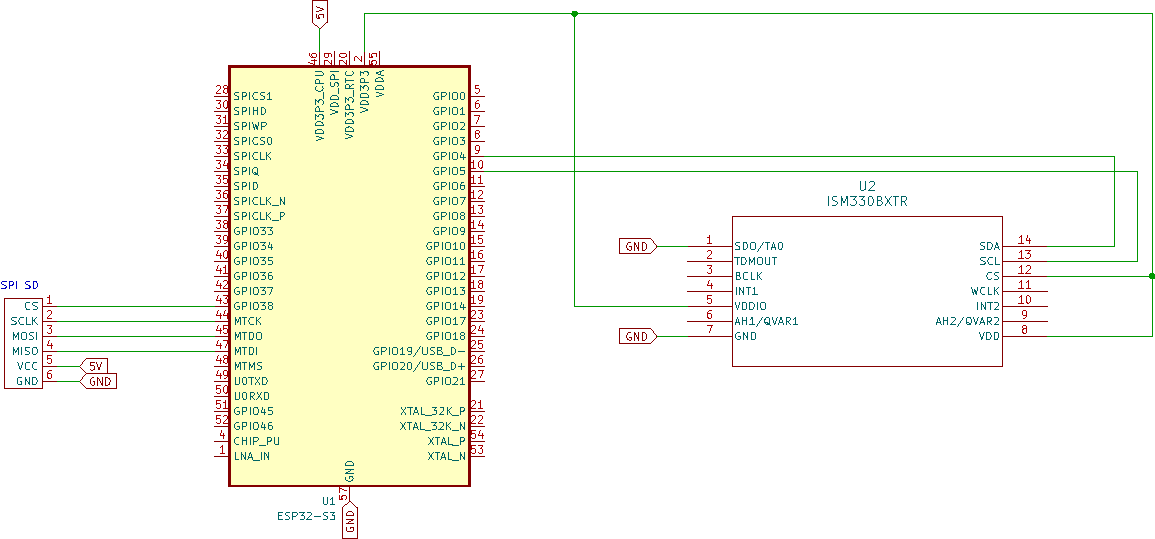
\includegraphics[width=0.95\textheight, height=0.8\textwidth, keepaspectratio]{assets/images/schematic.pdf}
	\caption{Schema logico}
	\label{fig:fullpage-schematic}
\end{sidewaysfigure}
\clearpage

\subsection{Consumo Energetico}

\begin{samepage}
\subsubsection{ESP32-S3 (Microcontrollore)}
\begin{table}[H]
	\centering
	\caption{ESP32-S3 Power Consumption -- CPU Active, \(25\,^\circ\mathrm{C}\)}
	\label{tab:esp32s3_cpu_power}
	\begin{tabularx}{\textwidth}{lccc}
		\hline
		\textbf{CPU Frequency} & \textbf{Peripherals} & \textbf{Data Access} & \textbf{Consumption} \\
		\hline
		$80\,\text{MHz}$  & $\times$     & $32$ bit  & $33.1\,\text{mA}$ \\
		$80\,\text{MHz}$  & \checkmark   & $32$ bit  & $47.3\,\text{mA}$ \\
		$80\,\text{MHz}$  & $\times$     & $128$ bit & $41.8\,\text{mA}$ \\
		$80\,\text{MHz}$  & \checkmark   & $128$ bit & $56.3\,\text{mA}$ \\
		$240\,\text{MHz}$ & $\times$     & $32$ bit  & $66.2\,\text{mA}$ \\
		$240\,\text{MHz}$ & \checkmark   & $32$ bit  & $81.3\,\text{mA}$ \\
		$240\,\text{MHz}$ & $\times$     & $128$ bit & $91.7\,\text{mA}$ \\
		$240\,\text{MHz}$ & \checkmark   & $128$ bit & $107.9\,\text{mA}$ \\
		\hline
	\end{tabularx}
\end{table}
\begin{table}[H]
	\centering
	\caption{ESP32-S3 Low-Power Modes, \(25\,^\circ\mathrm{C}\)}
	\label{tab:esp32s3_low_power}
	\begin{tabularx}{\textwidth}{lXc}
		\hline
		\textbf{Mode} & \textbf{Condition} & \textbf{Consumption} \\
		\hline
		Light-sleep & CPU e digital peripherals in clock-gating, Wi-Fi disattivato & $0.240\,\text{mA}$ \\
		Deep-sleep & RTC memory e RTC peripherals alimentati & $0.008\,\text{mA}$ \\
		\hline
	\end{tabularx}
\end{table}
\begin{table}[H]
	\centering
	\caption{ESP32-S3 Wi-Fi Power Consumption, \(25\,^\circ\mathrm{C}\)}
	\label{tab:esp32s3_wifi_power}
	\begin{tabularx}{\textwidth}{lXc}
		\hline
		\textbf{Mode} & \textbf{Configuration} & \textbf{Consumption} \\
		\hline
		Transmitter & $802.11\text{b}$, $1\,\text{Mbps}$, $P_{\text{OUT}}=+21\,\text{dBm}$ & $340\,\text{mA}$ \\
		Transmitter & $802.11\text{g}$, $54\,\text{Mbps}$, $P_{\text{OUT}}=+19\,\text{dBm}$ & $291\,\text{mA}$ \\
		Transmitter & $802.11\text{n}$, HT20, MCS7, $P_{\text{OUT}}=+18.5\,\text{dBm}$ & $283\,\text{mA}$ \\
		Transmitter & $802.11\text{n}$, HT40, MCS7, $P_{\text{OUT}}=+18\,\text{dBm}$ & $286\,\text{mA}$ \\
		Receiver & $802.11\text{b/g/n}$, HT20 & $88\,\text{mA}$ \\
		Receiver & $802.11\text{n}$, HT40 & $91\,\text{mA}$ \\
		\hline
	\end{tabularx}
\end{table}
\end{samepage}
Il profilo energetico usato é \textit{Modem-sleep mode}, rilasciato da Espressif \cite{esp32s3_datasheet}, dove il modem viene attivato solo quando necessario, quindi il consumo effettivo é:
\begin{itemize}
	\item in \textbf{Modem TX}: CPU Active/All RTC/Wi-Fi, durante la comunicazione dei dati (286 mA).
	\item in \textbf{Modem RX}: CPU Active/All RTC/Wi-Fi, durante la ricezione di modelli, comandi e configurazioni dei dati (91 mA).
	\item in \textbf{Modem sleep}: CPU Active/All RTC/No Wi-Fi, durante la fase di sola inferenza, scrittura su sd o lettura del sensore (81.3 mA).
\end{itemize}

Il sistema acquisisce campioni da \(12\,\mathrm{byte}\) (16bit per valore, 3 per accelerometro e 3 per giroscopio) ad una frequenza di
\(3.84\,\mathrm{kHz}\) (\(46.08\,\mathrm{kB/s}\)). I dati, convertiti in \textit{float32} (\(24\,\mathrm{byte}\) per campione), vengono trasmessi in blocchi da \(4096\) campioni.
La dimensione di ciascun blocco è quindi

\begin{equation}
	N_{\mathrm{TX}} = 4096 \cdot 24 = 98304\,\mathrm{byte}.
\end{equation}

Il periodo tra due trasmissioni in modalità \textit{continua}, ovvero vengono caricati tutti i \textit{datapoint}

\begin{equation}
	T_{\mathrm{block}} =
	\frac{4096}{3840}
	= 1.067\,\mathrm{s}.
\end{equation}

Assumendo la velocità teorica massima di \(150\,\mathrm{Mbit/s}\) per
802.11n HT40 MCS7, il tempo necessario per un blocco è

\begin{equation}
	T_{\mathrm{TX}} =
	\frac{98304\cdot8}{150\cdot10^6}
	= 5.24\,\mathrm{ms}.
\end{equation}

Assumendo una corrente di \(286\,\mathrm{mA}\) la potenza per singola trasmissione è

\begin{equation}
	E_{\mathrm{TX}}
	=
	\frac{3.3\cdot0.286\cdot5.24\times10^{-3}}{3.6}
	\approx
	\boxed{1.37\times10^{-3}\,\mathrm{mWh}}.
\end{equation}

Il duty cycle della trasmissione è

\begin{equation}
	D_{\mathrm{TX}} =
	\frac{5.24\,\mathrm{ms}}{1.067\,\mathrm{s}}
	\approx0.492\%.
\end{equation}

La corrente media associata al Wi-Fi è quindi

\begin{equation}
	I_{\mathrm{WiFi,avg}}
	=
	286\,\mathrm{mA}\cdot0.00492
	\approx1.41\,\mathrm{mA}.
\end{equation}

Considerando inoltre \(81.3\,\mathrm{mA}\) per CPU e periferiche attive, la corrente media complessiva risulta

\begin{equation}
	I_{\mathrm{avg}}
	=
	81.3+1.41
	\approx82.7\,\mathrm{mA}.
\end{equation}


I valori ottenuti rappresentano una stima teorica basata sulla velocità massima di \(150\,\mathrm{Mbit/s}\) e non tengono conto degli overhead del protocollo Wi-Fi e dei livelli superiori.


\begin{samepage}
\subsubsection{ISM330BX}

\begin{table}[H]
	\centering
	\small
	\begin{tabularx}{\textwidth}{l X r}
		\toprule
		\textbf{Modalità Operativa} & \textbf{Dettagli Canali e Funzionalità} & \textbf{Corrente Tipica ($I_{DD}$)} \\
		\midrule
		Combo High-Performance & Accelerometro + Giroscopio attivi ad alto ODR & $\approx \SI{0.60}{\milli\ampere}$ ($\SI{600}{\micro\ampere}$) \\
		Power-Down & Dispositivo spento, interfacce seriali in attesa & $\SI{3}{\micro\ampere}$ -- $\SI{5}{\micro\ampere}$ \\
		\bottomrule
	\end{tabularx}
	\caption{Consumi elettrici ISM330BX \cite{ism330bx_datasheet}.}
	\label{tab:ism330bx_power}
\end{table}
Il sensore viene usato in modalità \textit{High-Performance} a 3.84khz, con coda FIFO, ovvero il sensore salva in una regione di memoria le letture, il che permette di leggere a blocchi i dati dal sensore. Il firmware interroga il sensore chiedendo 512 byte alla volta.
\end{samepage}
\begin{samepage}

 \subsubsection{Adafruit 4682}
 Il breakout Adafruit 4682 è una scheda passiva, quindi il consumo é dato unicamente dalla scelta della scheda microsd.
Consumo scheda SD:
\begin{table}[H]
	\centering

	\label{tab:microsd-current}
	\begin{tabular}{lllcc}
		\hline
		Current &  $V_{\mathrm{DD}}$ & Max. \\
		\hline
		Peak
		& 3.6 V
		& 300 mA \\
		\hline
		Average
		& 3.6 V
		& 250 mA \\
		\hline
	\end{tabular}
		\caption{consumi di una scheda microSD, microSDXC, Class 10, U1, 64GB, modello SDCIT/64GB, marca Kingston \cite{kingston_industrial_microsd}.}
\end{table}

\end{samepage}


Analogamente al caso precedente, si riutilizzano gli stessi risultati per il
consumo del controllore. Considerando un data rate di
\(46.08\,\mathrm{kB/s}\), e una velocità minima di scrittura di
\(10\,\mathrm{MB/s}\) per una SD Classe 10, il duty cycle della scrittura o lettura è
pari a circa \(0.46\%\).

Assumendo un consumo di \(250\,\mathrm{mA}\) durante la scrittura o lettura il consumo
medio della SD è quindi circa \(1.15\,\mathrm{mA}\). Sommando il consumo
della CPU e delle periferiche, pari a \(81.3\,\mathrm{mA}\), si ottiene

\begin{equation}
	I_{\mathrm{avg,SD}}\approx82.45\,\mathrm{mA},
	\qquad
	P_{\mathrm{avg,SD}}\approx\boxed{272.1\,\mathrm{mW}}.
\end{equation}

\needspace{5\baselineskip}
\subsection{Sintesi dei Consumi di Sistema}
Sommando i consumi si ha un consumo medio teorico di $\approx83.75\mathrm{mA}$, o $\approx276.4\mathrm{mW}$, e un consumo di picco di $\approx 618.9\mathrm{mA}$ o $\approx2042\mathrm{mW}$.

Il che significa che una batteria 18650 da circa 9Wh, riuscirebbe ad alimentare il dispositivo per 32 ore.

\subsubsection{Tecniche di Ottimizzazione energetica}
La stima di 32 ore si riferisce all'autonomia con il massimo consumo, ovvero con continua lettura, salvataggio, invio dei dati e l'inferenza basata su suddetti dati.
Una volta che la \textit{backend} riceve abbastanza dati per allenare modelli validi si può mettere il device in varie modalità risparmio energetico configurabile. %circa lo supporta ma non proprio


\begin{table}[H]
	\centering
	\label{tab:esp32s3_duty_cycle}
	\begin{tabularx}{\textwidth}{lccccc}
		\hline
		\textbf{Modalità} & \textbf{CPU} & \textbf{Duty Cycle} & \textbf{Corrente} & \textbf{Potenza} & \textbf{Autonomia} \\
		\hline
		Active & $240\,\mathrm{MHz}$ & $100\%$ & $83.75\,\mathrm{mA}$ & $276.4\,\mathrm{mW}$ & $32.6\,\mathrm{h}$ \\
		Active & $80\,\mathrm{MHz}$ & $100\%$ & $49.75\,\mathrm{mA}$ & $164.2\,\mathrm{mW}$ & $54.8\,\mathrm{h}$ \\
		Light-sleep & $240\,\mathrm{MHz}$ & $3.33\%$ & $3.70\,\mathrm{mA}$ & $12.22\,\mathrm{mW}$ & $30.7\,\mathrm{giorni}$ \\
		Light-sleep & $80\,\mathrm{MHz}$ & $3.33\%$ & $2.57\,\mathrm{mA}$ & $8.48\,\mathrm{mW}$ & $44.2\,\mathrm{giorni}$ \\
		Deep-sleep & $240\,\mathrm{MHz}$ & $3.33\%$ & $3.48\,\mathrm{mA}$ & $11.47\,\mathrm{mW}$ & $32.7\,\mathrm{giorni}$ \\
		Deep-sleep & $80\,\mathrm{MHz}$ & $3.33\%$ & $2.34\,\mathrm{mA}$ & $7.74\,\mathrm{mW}$ & $48.5\,\mathrm{giorni}$ \\
		\hline
	\end{tabularx}
	\caption{Consumi e autonomia stimati nelle modalità, batteria da \(9\,\mathrm{Wh}\). Il duty cycle è del \(3.33\%\) (2 minuti di attività ogni ora, ovvero circa 112 segmenti da 4096 datapoint). Il duty cycle del Wi-Fi viene scalato a \(0.41\%\), il lettore SD è spento durante le fasi di sleep.}
\end{table}

\section{Software}
\subsection{Struttura principale}
Il codice del firmware é scritto in C/C++ usando il framework ESP-IDF.
Il sistema giova dell'architettura dual core del microcontrollore ESP32-S3 \cite{esp32s3_datasheet}.
Ci sono 6 task/thread principali.



\begin{table}[H]
	\centering
	\begin{tabularx}{\textwidth}{Xcc}
		\hline
		\textbf{Nome Task} & \textbf{Priorità} & \textbf{Core Assegnato} \\ \hline
		\texttt{harvester}   & 5                 & Core 1                  \\ \hline
		\texttt{inferencer}  & 4                 & Core 1                  \\ \hline
		\texttt{uploader}    & 3                 & Core 0                  \\ \hline
		\texttt{dump\_reader} & 3                 & Core 0                  \\ \hline
		\texttt{sd\_writer}   & 2                 & Core 0                  \\ \hline
		\texttt{mqtt\_task}  & 5 (Default)       & Core 0 (Default)        \\ \hline
	\end{tabularx}
	\caption{Priorità delle Task FreeRTOS e selezione Core}
	\label{tab:freertos_tasks}
\end{table}
Tutte le task nel core 0 hanno grandi ritardi di I/O perché richiedono chiamate di rete oppure la lettura e scrittura di file su scheda SD. Mentre l'inferencer nel Core 1 é cpu-bound per la maggior parte del tempo e IO-bound se deve caricare i modelli dalla rete oppure dalla scheda SD. L'harvester viene messo nello stesso Core dell'inferencer perché vogliamo dare precedenza alla lettura dei dati in maniera prioritaria.

\begin{description}
	\item[\texttt{harvester} (Core 1, Priorità 5)] Esegue l'interrogazione della coda FIFO del sensore ISM330BX via SPI per estrarre i campioni di accelerometro e giroscopio. La priorità é massima per permettere alla coda FIFO di non riempirsi mai e non andare in \textit{overrun} \cite{ism330bx_datasheet}, il che significherebbe perdere dei \textit{datapoints} contigui.

	\item[\texttt{inferencer} (Core 1, Priorità 4)] Calcola la magnitudo e carica dello spettrogramma STFT 2D. Esegue i modelli dell'\textit{ensemble} (insieme di modelli) e calcola il valore delle anomalie.

	\item[\texttt{uploader} (Core 0, Priorità 3)] Gestisce la serializzazione in formato CBOR e la trasmissione dei dati. Divide l'array di campioni float in pacchetti più piccoli per rientrare nei limiti dei buffer di rete dell'MQTT, e li invia al broker MQTT. %512 ma potrei cambiarlo


	\item[\texttt{dump\_reader} (Core 0, Priorità 3)] Viene istanziato temporaneamente in caso di trigger di replay, ovvero se la backend richiede un upload di tutti i dati storici salvati. Legge i file binari dalla scheda SD e li reinserisce nella pipeline di elaborazione, nello stesso modo in cui farebbe \textit{harvester}, che viene messo in pausa nel caso venga richiesto il replay. É un processo IO-bound, quindi messo nel Core 0.

	\item[\texttt{sd\_writer} (Core 0, Priorità 2)] Prende i dati (sia i datapoint che i risultati dell'inferenza) e li scrive sulla scheda SD in formato binario.

	\item[\texttt{mqtt\_task} (Core 0, Priorità 5 -- Default di Sistema)] Gestito in background dalla libreria client di MQTT di Espressif (\textit{espressif/mqtt} \cite{espressif_esp_mqtt}).
\end{description}

\subsection{4-way Buffer}
%citazione necessaria da trovare per il ping pong buffer.

La struttura dati principale che unisce le varie task é un \textit{4-way buffer}, una variante di un \textit{Ping Pong buffer} \cite{lyons2010dsp} con 4 buffer al posto di 2.
Tutte le task leggono e scrivono dagli slot del quad buffer, usando dei semafori per la sincronizzazione, e per evitare controlli attivi.

 \begin{figure}[H]
	\centering
	\begin{tikzpicture}[node distance=1.2cm, auto]

		\tikzstyle{state} = [draw=black, rectangle, rounded corners, minimum width=3.8cm, minimum height=1.2cm, align=center, thick, fill=white, font=\small]
		\tikzstyle{decision} = [draw=black, diamond, aspect=2, minimum width=3.8cm, minimum height=1cm, align=center, thick, fill=white, font=\small]
		\tikzstyle{flow} = [->, >=stealth, thick, draw=black]
		\tikzstyle{loopline} = [->, >=stealth, dashed, thick, draw=black!50]

		\node[state] (free) at (0,10.5) {\textbf{Slot Libero} };
		\node[state] (acq) at (0,8.6) {\textbf{Slot in Acquisizione} \\ \small (Preso da: \textbf{Harvester})};

		\node[decision] (dec) at (0,6.6) {Assegnamento slot};

		\node[state] (inf) at (-3.4,4.4) {\textbf{Slot in elaborazione} \\ \small (Acquisito da \textbf{Inferencer})};
		\node[state] (post_inf) at (-3.4,2.4) {\textbf{Slot elaborato}};

		\node[state] (bypass) at (3.4,3.4) {\textbf{Bypass elaborazione} \ };

		\node[state] (up_task) at (-2.4,-0.4) {\textbf{Slot pronto per Upload} \\ \small (Acquisito da \textbf{Uploader})};
		\node[state] (sd_task) at (2.4,-0.4) {\textbf{Slot pronto per SD} \\ \small (Acquisito da \textbf{SD Writer})};

		\draw[dashed, thick, black!70] (-5.4, 0.6) rectangle (5.4, -1.4);

		\node[font=\scriptsize\bfseries, black!70] at (0, 0.3) {ESECUZIONE CONCORRENTE };

		\node[state] (release) at (0,-3.2) {\textbf{Slot Rilasciato} };

		\draw[flow] (free) -- (acq);
		\draw[flow] (acq) -- (dec);

		\draw[flow] (dec.west) -| node[above, pos=0.5, font=\small] {Inferencer} (inf.north);
		\draw[flow] (dec.east) -| node[above, pos=0.5, font=\small] {Uploader \& SD} (bypass.north);

		\draw[flow] (inf) -- (post_inf);

		\coordinate (merge_point) at (0, 1.3);
		\coordinate (parallel_top) at (0, 0.6);

		\draw[thick] (post_inf.south) |- (merge_point);
		\draw[thick] (bypass.south) |- (merge_point);
		\draw[flow] (merge_point) -- (parallel_top);

		\draw[flow] (up_task.south) |- (release.west);
		\draw[flow] (sd_task.south) |- (release.east);

		\draw[loopline] (release.south) -- ++(0,-0.8) -- ++(-6.8,0) |- node[left, pos=0.9, font=\scriptsize, align=center] {Reinserito in\\free\_slots\_queue} (free.west);

	\end{tikzpicture}
	\caption{Grafo del ciclo di vita di uno slot in modalità continua}
	\label{fig:slot_lifecycle_fork_join_spaced}
\end{figure}


L'harvester prende il primo slot che trova quindi, dopo essere stato popolato dai dati, viene acquisito dall'inferencer, e poi sd\_writer e uploader salvano su sd e caricano sul cloud il segmento con i dati inferenziali ,oppure se l'inferencer sta elaborando un altro slot, viene assegnato direttamente al uploader e al sd\_writer, che salvano e caricano lo slot senza dati inferenziali.
La ragione per cui abbiamo bisogno di 4 buffer é che questo garantisce che 2 siano sempre occupati dal harvester che salva i dati come un classico ping pong buffer senza interruzioni, uno sia occupato dall'inferencer e un altro dai uploader e sd\_writer, in questo modo nessun task deve aspettarne un altro.

Il sistema é predisposto anche per altre modalità. Le modalità di upload di dati, configurabili dalla backend runtime sono:

\begin{itemize}
	\item \textit{Continuous}: ovvero quello nel grafico sopra, il device carica sul cloud tutti i dati che riesce, elaborati o no.
	\item \textit{AnomalyOnly}: il device carica sul cloud il segmento solo se risulta in un anomalia.
	\item \textit{AnomalyOrPeriodic}: il device carica sul cloud il segmento solo se risulta in un anomalia, ma carica con una certa cadenza anche dati non anomali per permettere un allenamento continuo dei modelli.
	\item \textit{ContinuousScoreRawAnomaly}: il device carica sempre il risultato dell'inferenza, ma carica anche il segmento solo se si tratta di un anomalia.
\end{itemize}

Il device espone alla backend dei comandi di dump opzionali, questi sono \textit{dump}, che carica sul cloud tutti i dati dalla scheda SD senza farne l'inferenza (harvester e inferencer disabilitati) e \textit{dump\_i} che carica tutti i dati, ma calcolandone anche le anomalie (harvester disabilitato).

Nella configurazione del device é possibile anche disabilitare del tutto la scheda sd per risparmiare energia se non si ha bisogno di chiamare il comando \textit{dump} dei dati.

\section{Inferencer}
L'inferencer è la task che gestisce la vita dei modelli e la loro inferenza, appoggiandosi ad una struttura dati chiamata \textit{ensemble} che aiuta la gestione dei modelli e astrae l'utilizzo della libreria tflite micro \cite{espressif_esp_tflite_micro}.
Ai dati viene applicata una pipeline che riduce la dimensionalità, ovvero una riduzione euclidea di magnitudo per accelerazione e giroscopio:

\begin{samepage}

$$\text{Accel Magnitude}[n] = \sqrt{\text{accel}_x[n]^2 + \text{accel}_y[n]^2 + \text{accel}_z[n]^2}$$

$$\text{Gyro Magnitude}[n] = \sqrt{\text{gyro}_x[n]^2 + \text{gyro}_y[n]^2 + \text{gyro}_z[n]^2}$$
\end{samepage}
questo permette di mantenere solo i dati vibrazionali, indipendentemente dall'orientamento di montaggio del sensore.

Successivamente viene applicata ad entrambi una funzione a finestra di hanning (overlap 75\%) e una trasformazione di Fourier.
Viene scelta la finestra di Hanning perchè offre un buon compromesso tra risoluzione e contenimento dello spectral leakage \cite{harris1978use}.


\begin{figure}
	\centering
	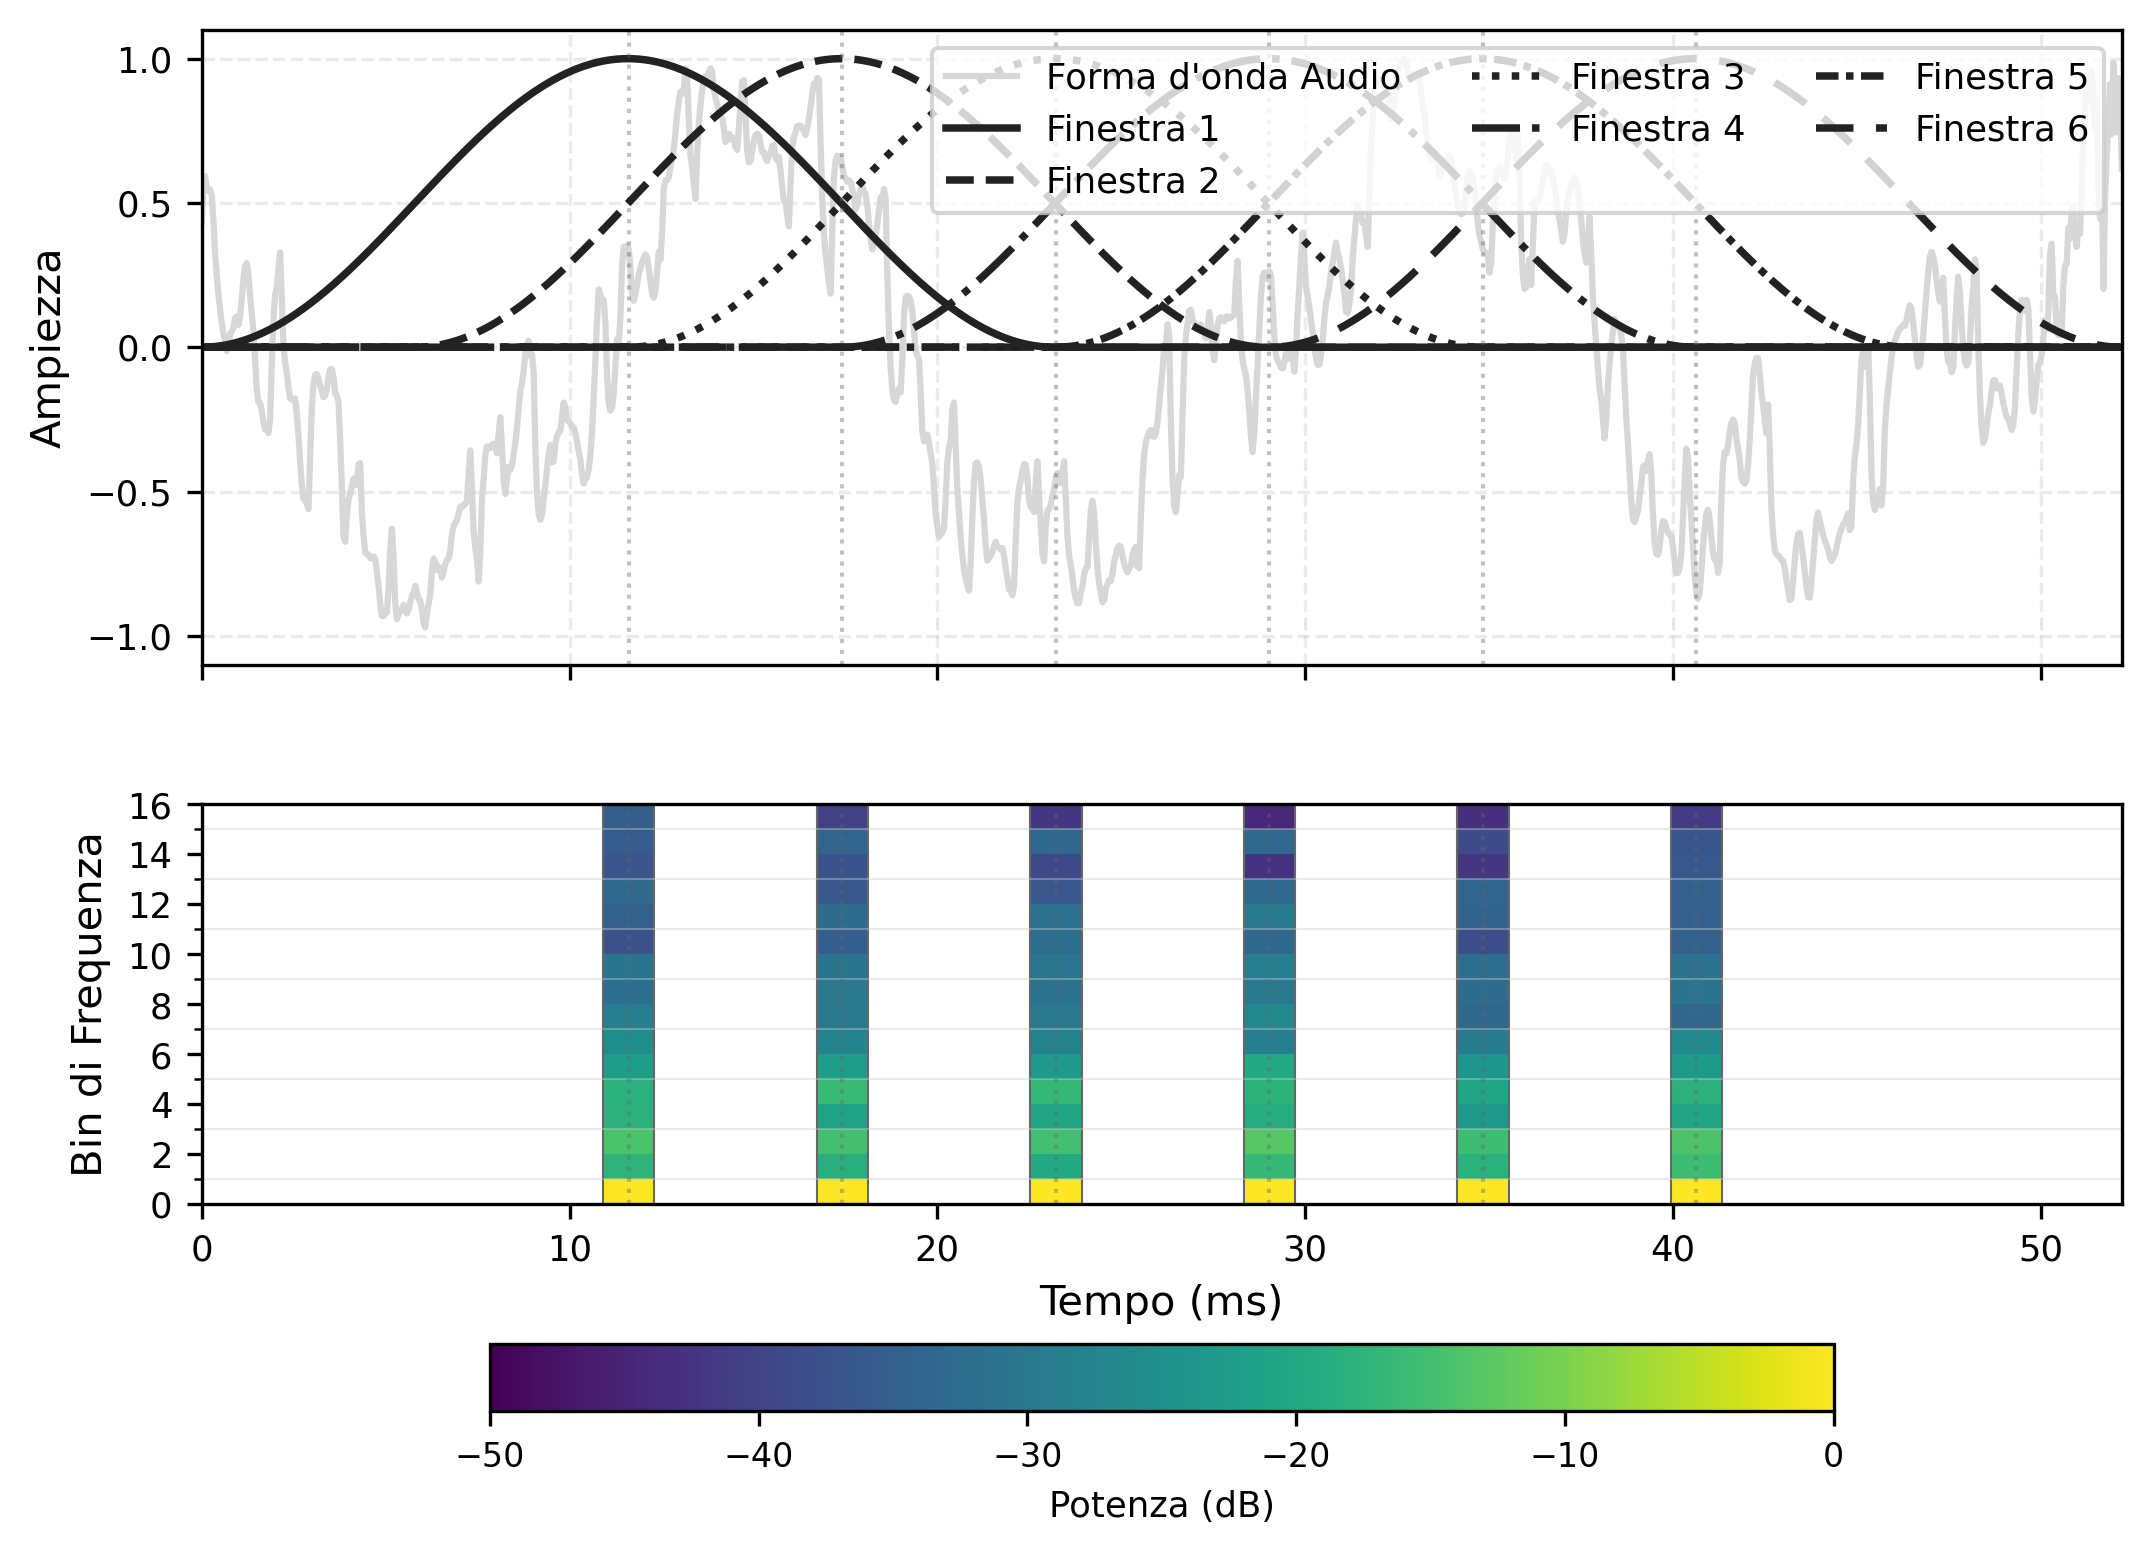
\includegraphics[width=1\linewidth]{assets/images/stft}
	\caption{Applicazione finestra di hanning e trasformata di fourier}
	\label{fig:stft}
\end{figure}

Infine gli spettrogrammi STFT del giroscopio e accelerazione vengono concatenati lungo l'asse delle feature di frequenza, così da creare un solo segmento di dati.

\subsection{Architettura dell'\textit{ensemble}}
L'architettura è formata da 3 tipi di modelli disposti in maniera simil-MIXAE \cite{mixae_zhang2017deep}:


\begin{figure}[H]
	\centering
	\resizebox{\textwidth}{!}{%
		\begin{tikzpicture}[
			>=Stealth,
			box/.style={
				draw,
				thick,
				fill=white,
				minimum width=2.4cm,
				minimum height=1.15cm,
				align=center,
				rounded corners=2pt,
				font=\sffamily
			},
			imgbox/.style={
				draw,
				thick,
				inner sep=0pt,
				fill=white
			},
			stackbox/.style={
				draw,
				thick,
				fill=white,
				minimum width=2cm,
				minimum height=2cm
			},
			solid arr/.style={
				thick,
				->,
				rounded corners=3pt
			},
			dashed arr/.style={
				dashed,
				thick,
				->,
				rounded corners=3pt
			},
			double line/.style={
				double,
				double distance=2pt,
				thick,
				rounded corners=3pt
			},
			font=\sffamily
			]

			% Input
			\coordinate (in_pos) at (0,0);

			\node[stackbox, shift={(-6pt,6pt)}] at (in_pos) {};
			\node[stackbox, shift={(-3pt,3pt)}] at (in_pos) {};

			\node[imgbox] (input) at (in_pos)
			{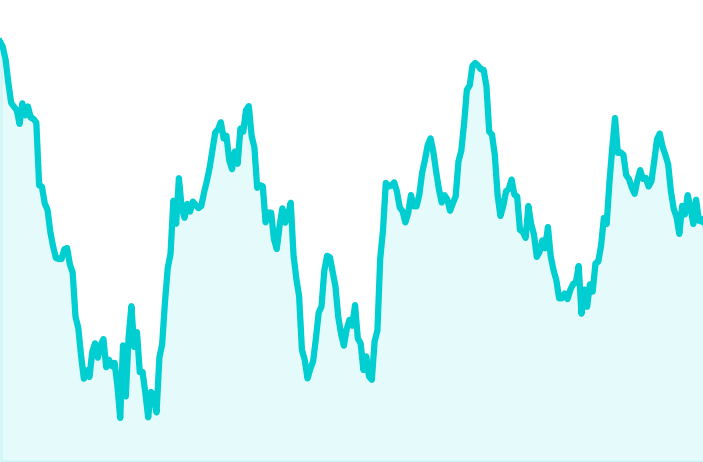
\includegraphics[
				width=2cm,
				height=2cm
				]{assets/images/waveform.png}};

			\node[below=0.15cm of input, font=\small] {Input};

			% STFT
			\node[imgbox] (stft) at (3.5,0)
			{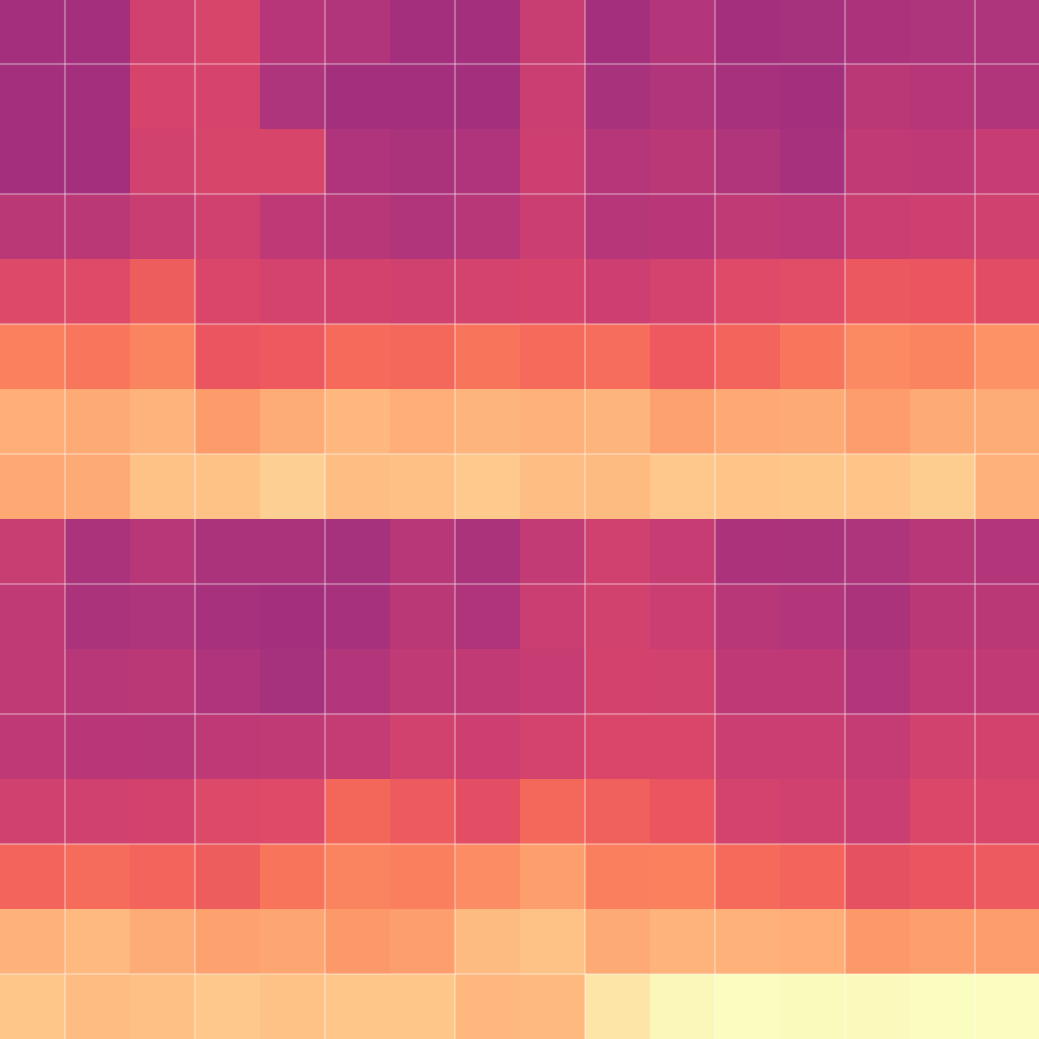
\includegraphics[
				width=2cm,
				height=2cm
				]{assets/images/spectrogram3.png}};

			\node[below=0.15cm of stft, font=\small] {STFT};

			\draw[solid arr]
			(input.east) -- (stft.west);

			% Router e Memoria
			\node[box] (router) at (7.0,1.6) {Router};
			\node[box] (memory) at (7.0,-1.6) {Memoria};

			% Split principale dopo STFT (Est)
			\coordinate (stft_split) at (5.2,0);

			\draw[thick]
			(stft.east) -- (stft_split);

			% STFT -> Router
			\draw[solid arr]
			(stft_split)
			-- (5.2,1.6)
			-- (router.west);

			% STFT -> Memoria
			\draw[solid arr]
			(stft_split)
			-- (5.2,-1.6)
			-- (memory.west);

			% Memoria -> Router (concat)
			\draw[dashed arr]
			(memory.north)
			-- (router.south)
			node[midway,right,font=\footnotesize] {concat};

			% Modelli
			\node[box] (mod1) at (12.5,1.6) {Modello 1};
			\node[font=\Huge] (dots) at (12.5,0) {$\vdots$};
			\node[box] (modN) at (12.5,-1.6) {Modello $N$};

			% Ingressi Modello 1: STFT (alto), Router (centro), Memoria (basso)
			\coordinate (m1_stft)   at (11.3,1.76);
			\coordinate (m1_router) at (11.3,1.60);
			\coordinate (m1_mem)    at (11.3,1.44);

			% Ingressi Modello N: STFT (alto), Memoria (centro), Router (basso)
			\coordinate (mN_stft)   at (11.3,-1.44);
			\coordinate (mN_mem)    at (11.3,-1.60);
			\coordinate (mN_router) at (11.3,-1.76);

			% Router -> modelli (Trunk a x=9.5)
			\coordinate (router_split) at (9.5,1.6);

			% Verso Modello 1 (dritto al centro: y=1.60)
			\draw[double line, ->]
			(router.east) -- (router_split) -- (m1_router);

			% Verso Modello N (scende alla porta inferiore: y=-1.76)
			\draw[double line, ->]
			(router.east) -- (router_split) |- (mN_router);

			% STFT -> Modelli e snstruction Error (percorso inferiore)
			\coordinate (model_recon_split) at (10.0,-4.2);

			% Da stft_split scende a -4.2 e va a destra fino allo split
			\draw[thick]
			(stft_split) -- (5.2,-4.2) -- (model_recon_split);

			% STFT -> Modello 1 (Porta superiore: y=1.76)
			\draw[solid arr]
			(model_recon_split)
			-- (10.0,1.76)
			-- (m1_stft);

			% STFT -> Modello N (Porta superiore: y=-1.44)
			\draw[solid arr]
			(model_recon_split)
			-- (10.0,-1.44)
			-- (mN_stft);

			% Memoria -> modelli (Trunk a x=10.5)
			% Linea perfettamente orizzontale da memory.east (y=-1.60) fino a x=10.5
			\coordinate (memory_split) at (10.5,-1.6);

			\draw[dashed,thick]
			(memory.east) -- (memory_split);

			% Da x=10.5 sale verso Modello 1 (Porta inferiore: y=1.44)
			\draw[dashed arr]
			(memory_split)
			-- (10.5,1.44)
			-- (m1_mem);

			% Da x=10.5 va dritto verso Modello N (Porta centrale: y=-1.60)
			\draw[dashed arr]
			(memory_split) -- (mN_mem);

			% Output
			\node[imgbox] (output) at (16.0,1.6)
			{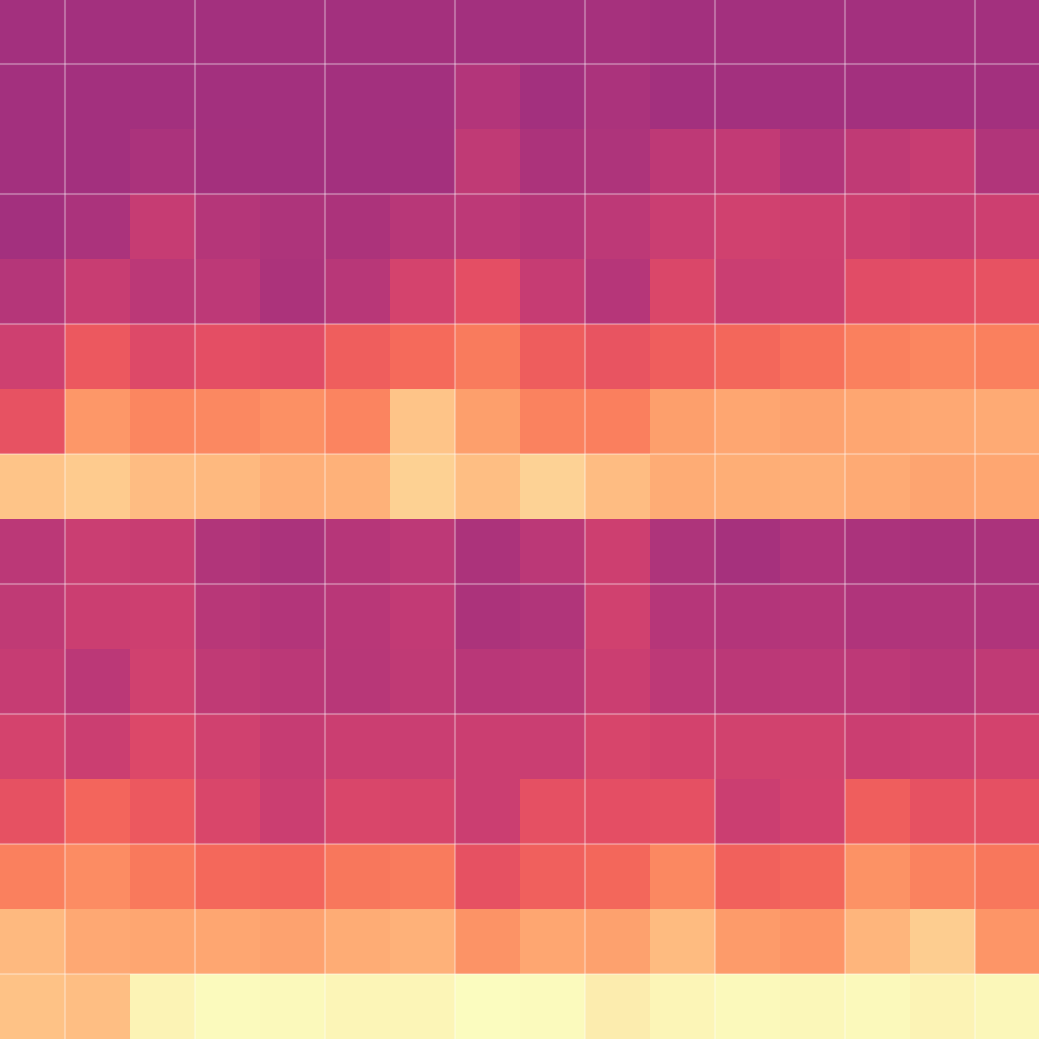
\includegraphics[
				width=2cm,
				height=2cm
				]{assets/images/spectrogram4.png}};

			\node[below=0.15cm of output, font=\small]
			{Output Selezionato};

			\draw[solid arr]
			(mod1.east) -- (output.west);

			% Reconstruction Error
			\node[
			box,
			fill=gray!10
			] (recon) at (16.0,-4.2)
			{Errore di \\ ricostruzione};

			% STFT -> Reconstruction Error (collegamento diretto orizzontale)
			\draw[solid arr]
			(model_recon_split) -- (recon.west);

			% Output -> Reconstruction Error
			\draw[solid arr]
			(output.south)
			-- (output.south |- recon.north)
			-- (recon.north);

			% Legenda
			\node[
			draw,
			thick,
			rounded corners=2pt,
			fill=white,
			align=left,
			inner sep=6pt,
			font=\footnotesize
			] at (7.5,-5.85)
			{%
				\textbf{Legenda}\\[3pt]
				\tikz[baseline=-0.5ex]
				\draw[thick,->] (0,0) -- (0.8,0);
				\quad Flusso principale\\[4pt]
				\tikz[baseline=-0.5ex]
				\draw[double,double distance=2pt,thick,->]
				(0,0) -- (0.8,0);
				\quad Selezione modello (argmax)\\[4pt]
				\tikz[baseline=-0.5ex]
				\draw[dashed,thick,->] (0,0) -- (0.8,0);
				\quad Memoria (opzionale)
			};

		\end{tikzpicture}%
	}
	\caption{Architettura del \textit{ensemble}.}
	\label{fig:architecture}
\end{figure}


\begin{itemize}
	\item 1 \textbf{Router}: prende in input un segmento e lo stato della memoria e decide quale autoencoder dovrà processarlo.
	\item 1 \textbf{Memoria}: memoria, opzionale per modello. Utile per modelli non convoluzionali, è un modo per aggiungere informazioni sul passato.
	\item N \textbf{autoencoder}: ci sono N (max 16), autoencoder che prendono il segmento e provano a ricostruirlo, l'errore di ricostruzione indica il livello di anomalia, configurabile tra MSE lineare e MSE logaritmico, può essere usato qualsiasi modelli rappresentabile con grafi nativi tflite micro.

\end{itemize}


\subsection{Gestione dei sottomodelli}
In memoria non possono alloggiare tutti i sottomodelli, se si scelgono architetture troppo complesse, quindi è necessario avere un modo di caricare a bisogno i sottomodelli.
Per questo l'inferencer dispone di una struttura dati di cache di modelli, creando così una gerarchia di recupero dati. Prima viene interrogata la cache alla ricerca del modello, poi la scheda sd se abilitata, poi il cloud attraverso una richiesta MQTT.
Una volta caricato un nuovo modello, se la memoria non è sufficiente, viene rimosso il modello usato meno recentemente, liberando così una parte di memoria.


% aggiungere sdw writer, harvester, uploader e dump_reader? non c'è tanto altro da dire

\section{Ottimizzazioni}
Vengono usate varie funzioni ottimizzate per l'ESP32S3.
\begin{itemize}
	\item \textbf{dsp\_opt\_int16\_to\_float}, custom, permette di convertire un buffer da int16
	a float con l'istruzione FLOAT.S di Xtensa LX7 \cite{xtensa_isa}.
	 \item \textbf{\texttt{dsps\_fft2r\_fc32} (Radix-2 Complex FFT)}: calcola la fft sui dati del sensore. Fornita da ESP-DSP \cite{espdsp}.
	\item \textbf{\texttt{dsps\_fft2r\_init\_fc32} (Inizializzazione FFT)}: Precalcola le tabelle dei fattori rotazionali (\textit{twiddle factors}) per evitare runtime calcoli di seni e coseni, molto pesanti. Fornita da ESP-DSP \cite{espdsp}.
	\item \textbf{\texttt{dsps\_bit\_rev\_fc32} (Bit Reversal)}: Esegue il riordinamento dell'array in output di dsps\_fft2r\_fc32. Fornita da ESP-DSP \cite{espdsp}.
	\item \textbf{\texttt{dsps\_wind\_hann\_f32} (Generazione Finestra di Hanning)}: Calcola e applica la finestra di Hann. Fornita da ESP-DSP \cite{espdsp}.
	\item \textbf{\texttt{dsps\_mulc\_f32} (Moltiplicazione Vettore-Scalare)}: Esegue la moltiplicazione di un array float per un numero. Fornita da ESP-DSP \cite{espdsp}.
\end{itemize}


\subsection{Ottimizzazione della conversione in float}
\label{subsec:dsp_optimization}
Il sensore restituisce dati in tipo int16, ma le funzioni di calcolo si aspettano dati in formato float da -1 a 1, quindi dobbiamo convertirli usando la funzione dsp\_opt\_int16\_to\_float che sfrutta l'istruzione assembly FLOAT.S.

\subsubsection{L'istruzione \texttt{FLOAT.S}}
L'approccio \textit{naive} sarebbe fare un ciclo for facendo un cast di ogni valore del buffer in float e poi moltiplicarlo per $1/32768.0$:
\begin{equation}
	x_{\text{float}} = \text{(float)}x_{\text{int16}} \cdot \frac{1}{32768.0}
\end{equation}
Questo approccio fa eseguire nell'FPU del controllore due istruzioni: un cast hardware (\texttt{FLOAT.S} con fattore di scala nullo) ed una moltiplicazione in floating point (\texttt{MUL.S}).

Per ottimizzare si è sfruttato l'ISA del coprocessore matematico dell'architettura Xtensa LX7 dell'ESP32-S3. Come scritto nel manuale dell'ISA \cite{xtensa_isa},
 \texttt{FLOAT.S} possiede un campo per fare lo shift del risultato:
\begin{equation}
	\text{FR}[r] \leftarrow \text{floats}(\text{AR}[s]) \cdot 2^{-t} \quad \text{con } t \in [0, 15]
\end{equation}
Impostando $t = 15$, la FPU procede col casting int16-float e la divisione per $2^{15} = 32768$ nello stesso ciclo di clock. Si
elimina così l'istruzione di moltiplicazione e l'overhead di memoria per la costante.

\subsubsection{Ottimizzazione della pipeline}
Come definito nei modelli di schedulazione di GCC per l'architettura
Xtensa \cite{gcc_xtensa}, le istruzioni di caricamento sulla memoria \texttt{load} e di conversione (\texttt{fconv}) hanno latenze:
\begin{itemize}
	\item \textbf{Caricamento (\texttt{xtensa\_memory})}: 2 cicli di clock.
	\item \textbf{Conversione (\texttt{xtensa\_fconv})}: 2 cicli di clock (fully-pipelined, con throughput di 1 istruzione per ciclo).
\end{itemize}
Quindi se viene eseguita la conversione con FLOAT.S elemento per elemento, ovvero con fattore di unrolling U=1, la cpu dovrà continuare ad aspettare che la FPU scriva i risultati nei registri prima di poter salvare il valore in memoria.
Per evitare la latenza di pipeline abbiamo bisogno di un fattore di unrolling U maggiore uguale della latenza di pipeline \cite{patterson_hennessy}.

La latenza che abbiamo è di 4 cicli (2 di caricamento+2 di conversione), Quindi scegliamo U=4.


Lo pseudocodice dell'algoritmo ottimizzato con inline assembly è riportato nel Codice \ref{lst:dsp_opt_s3_assembly}.
\begin{lstlisting}[
	language=C,
	caption={Algoritmo di conversione ottimizzato a 4 vie con assembly Xtensa},
	label=lst:dsp_opt_s3_assembly,
	frame=single,
	basicstyle=\small\ttfamily,
	keywordstyle=\color{blue},
	commentstyle=\color{gray},
	breaklines=true,
	tabsize=2,
	keepspaces=true
	]
	void dsp_opt_int16_to_float(const int16_t *src, float *dest,
			int len) {
		int i = 0;
		for (; i + 3 < len; i += 4) {
			// genera istruzioni L16SI,
			// carica e converte in 2 cicli
			int32_t s0 = src[i+0]; int32_t s1 = src[i+1];
			int32_t s2 = src[i+2]; int32_t s3 = src[i+3];
			float f0, f1, f2, f3;

			asm volatile (
			"float.s %[f0], %[s0], 15 \n\t"
			"float.s %[f1], %[s1], 15 \n\t"
			"float.s %[f2], %[s2], 15 \n\t"
			"float.s %[f3], %[s3], 15"
			: [f0] "=f" (f0), [f1] "=f" (f1), [f2] "=f" (f2),
					[f3] "=f" (f3)
			: [s0] "r" (s0), [s1] "r" (s1), [s2] "r" (s2),
					[s3] "r" (s3)
			);

			dest[i+0] = f0; dest[i+1] = f1;
			dest[i+2] = f2; dest[i+3] = f3;
		}
	}
\end{lstlisting}

\subsubsection{Validazione sperimentale benchmark}
Per validare l'analisi è stato condotto un benchmark sull'ESP32-S3 misurando i cicli di clock effettivi tramite il registro \texttt{CCOUNT}.
Ogni benchmark è stato fatto su 20000 volte un buffer da 4096 valori, per simulare il vero utilizzo.


\begin{table}[H]
	\centering
	\begin{tabular}{lcccc}
		\toprule
		\textbf{Configurazione} & \textbf{Cicli/op} & \textbf{Tempo buffer} & \textbf{Ottimizzazione} & \textbf{Speedup} \\
		\midrule
		Assembly x1  & 17.08 & $291.50\,\mu\text{s}$ & $29.24\%$ & $1.41\times$ \\
		Assembly x2  & 10.57 & $180.39\,\mu\text{s}$ & $56.21\%$ & $2.28\times$ \\
		\textbf{Assembly x4} & \textbf{8.26} & $\mathbf{140.97\,\mu\text{s}}$ & $\mathbf{65.78\%}$ & $\mathbf{2.92\times}$ \\
		Assembly x8  &  9.01 & $153.77\,\mu\text{s}$ & $62.68\%$ & $2.68\times$ \\
		\midrule
		Naive C x1   & 24.14 & $411.99\,\mu\text{s}$ & $0.00\%$  & $1.00\times$ \\
		Naive C x2   & 17.58 & $300.03\,\mu\text{s}$ & $27.17\%$ & $1.37\times$ \\
		Naive C x4   & 14.32 & $244.39\,\mu\text{s}$ & $40.68\%$ & $1.68\times$ \\
		Naive C x8   & 12.82 & $218.79\,\mu\text{s}$ & $46.90\%$ & $1.88\times$ \\
		Naive C x16  & 11.95 & $203.95\,\mu\text{s}$ & $50.50\%$ & $2.02\times$ \\
		Naive C x32  & 22.55 & $384.85\,\mu\text{s}$ & $6.59\%$  & $1.07\times$ \\
		Naive C x64  & 23.34 & $398.29\,\mu\text{s}$ & $3.33\%$  & $1.03\times$ \\
		\bottomrule
	\end{tabular}
	\caption{Risultati del benchmark su ESP32-S3 a 240 MHz}
	\label{tab:fpu_benchmark_results}
\end{table}

Si può notare che il metodo più veloce è Assembly con U=4, il che conferma l'analisi teorica.
Si può anche notare che il metodo naive più veloce è con U=16, questo perchè la pipeline di calcolo naive è lunga 9 cicli perchè viene scomposta in 4 istruzioni, ovvero L16SI (2 cicli), FLOAT.S (2 cicli, senza shift), MUL.S (4 cicli), SSI (Store Single Precision, 1 ciclo), per un totale di 9 cicli totali. U deve essere quindi maggiore o uguale a 9, tuttavia per allineamento alla dimensione del bus, usiamo la potenza di due maggiore più vicina, ovvero 16.



